\section{Pola wektorowe}

\begin{definition}
  Niech $M$ będzie gładką rozmaitością. Gładką funkcję $X:M\to TM$ taką, że dla każdego $p\in M$ $X(p)\in T_pM\subseteq TM$ nazywamy \important{gładkim polem wektorowym} na $M$.

  Równoważnie możemy postawić warunek, że $\pi\circ X=id_M$.
\end{definition}

Często zamiast $X(p)$ piszemy krócej $X_p$, co oznacza wektor pola w punkcie $p$. \marginpar{Uogólnienie pól wektorowych pojawiających się w kontekście równań różniczkowych.}Pozwala to również uniknąć konfliktu notacji z pochodną kierunkową funkcji $f$ wzdłuż wektora $X$ ($Xf$).
  

\begin{center}
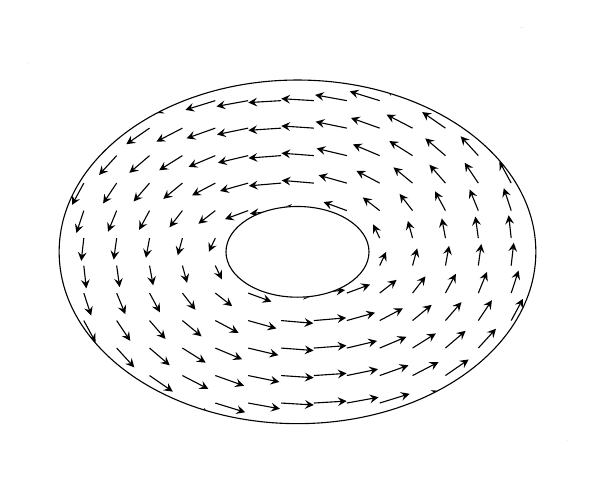
\begin{tikzpicture}[even odd rule]
%  \draw[rounded corners=35pt] (6.5,-1.8)--(2,-2)--(0,0) -- (2,2)--(4.2,1.4)--cycle;
%  \draw (3.5, 0.2) arc (-20:-130:0.9 and 0.7);
%  \draw (2.3, -0.15) arc (180:40:0.6 and 0.3);
%
%  \draw[thick, ->] (1.1, 0)--(1.4, 0.6);
%  \draw[thick, ->] (1.5, -0.6)--(1.6, 0.2);
%  \draw[thick, ->] (1.2, 0.8)--(2, 1.4);
%  \draw[thick, ->]  

\begin{axis}[%
  view     = {0}{90}, % for a view 'from above'
  domain   = -3:3,
  y domain = -3:3,
  %xtick    = {-3,...,3},
  %ytick    = {-3,...,3},
  axis line style={draw=none},
  ticks=none
  %tick style={draw=none}
]
\addplot3[
        quiver = {
            u = {-y/sqrt(x^2+y^2)},
            v = {x/sqrt(x^2+y^2+3)},
            scale arrows = 0.4,
        },
        -stealth,
        domain = -3:3,
        domain y = -3:3,
        samples=16
    ] {0};
%\addplot3[blue, quiver={u=8*x, v=2*y, scale arrows=0.05}, samples=16, -latex] (x,y,0);

  %\fill[clip, overlay=false, fill=white, color=white, fill opacity=0.5] (-4, 3.5) rectangle (5, -3.5) ellipse (0, 0) (1 and 0.5);

  \fill[preaction={clip}, fill=white] (-4,-3.5) rectangle (4,3.5) (0,0) ellipse (2.9 and 2.5);
  \draw (0,0) ellipse (2.9 and 2.5);
  \filldraw[white] (0,0) ellipse (0.84 and 0.66);
  \draw (0,0) ellipse (0.87 and 0.66);
 
\end{axis}
\end{tikzpicture}
\end{center}

Wyraźmy pole wektorowe $X:M\to TM$ w mapach $(U,\phi)$ na $M$ oraz $(TU,\overline{\phi})$ na $TM$. Niech $a_i:\phi(U)\to\R$ będą gładkimi funkcjami rzeczywistymi (nazwiemy je \acc[i]{współrzędnymi $X$} w mapach $\phi$ i $\overline{\phi}$) takimi, że
$$\overline{\phi}X\phi^{-1}(x)=(\;x,\;a_1(x),...,a_n(x)\;)=(\;x,\;\sum a_i(x)e_i\;),$$
gdzie $e_i$ to baza standardowa $\R^n$. Zgodnie z oznaczeniem z poprzedniego rozdziału $\frac{\partial}{\partial \phi_i}(p)=(\phi^*_p)^{-1}(e_i)$ mamy
$$X(p)=\sum a_i(\phi(p))\cdot\frac{\partial}{\partial\phi_i}(p).$$
Jeśli teraz oznaczymy $b_i=a_\circ\phi:U\to\R$, to wówczas
$$X(p)=\sum b_i(p)\cdot\frac{\partial}{\partial\phi_i}(p).$$

\begin{fact}
  Pole $X:M\to TM$ jest gładkim polem wektorowym na $M$ $\iff$ w mapie $(U,\phi)$ na $M$ i odpowiadającej jej mapie $(TU,\overline{\phi})$ na $TM$ wyraża się jako
  $$X(p)=\sum b_i(p)\cdot\frac{\partial}{\partial\phi_i}(p)$$
  dla pewnych gładkich $b_i:U\to\R$.
\end{fact}

\begin{proof}
  Bezpośrednio z przestawienia $X$ w mapach $(U,\phi)$ i $(TU,\overline{\phi})$ jak wyżej.
\end{proof}

Pole wektorowe na otwartym $U\subseteq\R^n$ ma postać
$$X(x)=\sum_{i\leq n}a_i(x)\cdot\frac{\partial}{\partial x_i}(x)$$
dla pewnych gładkich funkcji $a_i:U\to\R$. Z tego powodu będziemy pisać
$$X(x)=[a_1(x),...,a_n(x)]\in \R^n\cong T_xU.$$
Zjawiska lokalne dla pól na rozmaitościach będziemy wyrażać za pośrednictwem map za pomocą pól na otwartych podzbiorach $\R^n$.

\begin{conclusion}\label{wniosek 5:3}
  Suma dwóch gładkich pól wektorowych
  $$(X+Y)(p):=X(p)+Y(p)$$
  jest gładkim polem wektorowym.

  Iloczyn gładkiej funkcji $f:M\to\R$ oraz gładkiego pola $X$
  $$(f\cdot X)(p):=f(p)\cdot X(p)$$
  jest gładkim polem wektorowym
\end{conclusion}

Rodzinę wszystkich gładkich pól wektorowych na $M$ będziemy oznaczać przez $C^\infty(TM)$ lub $\color{blue}\mathfrak{X}(M)$. W algebraicznym rozumienia jest to moduł nad pierścieniem $C^\infty(M)$ gładkich funkcji rzeczywistych na $M$ (patrz wniosek \ref{wniosek 5:3}).

\subsection{Definiowanie pola wektorowego za pomocą rozkładów jedności}

Niech $M$ będzie rozmaitością z niepustym brzegiem $\partial M$. 

\begin{definition}
  Mówimy, że wektor $Y\in T_pM$, gdzie $p\in\partial M$, jest \important{skierowany do wewnątrz} $M$, jeśli w pewnej mapie $\phi:U_p\to H^n$ wyraża się przez
  $$Y=\sum_{i\leq n}a_i\cdot\frac{\partial}{\partial\phi_i}(p),\quad a_n>0$$
\end{definition}

\begin{fact}
  Jeśli wektor o początku $p$ jest skierowany do wewnątrz w jednej mapie, to jest tak w każdej innej mapie wokół $p$. Ponadto, suma wektorów skierowanych do wewnątrz jest wektorem skierowanym do wewnątrz.
\end{fact}

\begin{proof}
  Niech $Y$ będzie wektorem skierowanym do wewnątrz w mapie $(U,\phi)$. Niech $(V, \psi)$ będzie inną mapą wokół $p$. Wiemy, że
  $$Y=\sum a_i\cdot\frac{\partial}{\partial\phi_i}(p)$$
  i $a_n>0$. Chcemy teraz sprawdzić, co się dzieje w indeksie $n$, gdy przedstawimy ten wektor jako kombinację liniową $\frac{\partial}{\partial\psi_i}(p)$. Popatrzmy na zamianę baz:
  \begin{align*}
    \frac{\partial}{\partial\phi_n}(p)&=(\phi^*_p)^{-1}(e_n)=\\
        &=(\psi_p^*)^{-1}[\psi_p^*(\phi_p^*)^{-1}](e_n)=\\
        &=(\psi_p^*)^{-1}d\psi_p d(\phi)^{-1}_{\phi(p)}(e_n)=\\
        &=(\psi_p^*)^{-1}[d(\psi\phi^{-1})_{\phi(p)}(e_n)]
  \end{align*}
  Wiemy, że $\psi\phi^{-1}:\R^n\to\R^n$ jest funkcją rzeczywistą, czyli 
  $$d(\psi\phi^{-1})_{\phi(p)}=D_{\phi(p)}(\psi\phi^{-1})$$
  jest jej pochodną. Dodatkowo, wiemy, że $\psi\phi^{-1}$ jest bijekcją, więc na pewno $D_{\phi(p)}(\psi\phi^{-1})(e_n)$ nie może się zerować. Zarówno $\psi$ jak i $\phi$ są mapami wokół brzegu $\partial M$, czyli tak naprawdę:
  $$\psi\phi^{-1}:H^n\to H^n$$
  W takim razie, $D_{\phi(p)}(\psi\phi^{-1})(e_n)\in \{(x_1,...,x_n)\in\R^n\;:\;x_n>0\}$.% i 
  %$$a_n\cdot\frac{\partial}{\partial\phi_n}(p)=\underbrace{a_n\cdot D_{\phi(p)}(\phi\psi^{-1})(e_n)}_{>0}\cdot\frac{\partial}{\partial\psi_n}$$

  \begin{center}
  \scalebox{0.6}{
  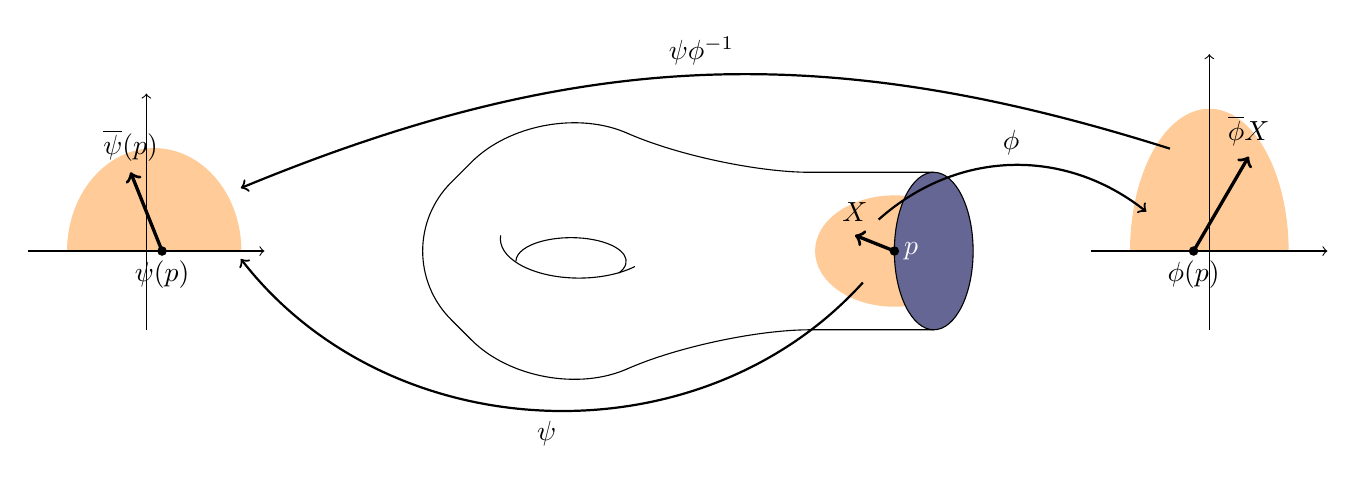
\begin{tikzpicture}
    \filldraw[orange!40] (6.5, 0) ellipse (1 and 0.7);
    \draw[->, very thick] (6.5, 0)--(6, 0.2);
      \draw[rounded corners=35pt](7,-1)--(4.2,-1)--(2,-2)--(0,0) -- (2,2)--(4.2,1)--(7,1);
      \draw (1.5,0.2) arc (175:315:1cm and 0.5cm);
      \draw (3,-0.28) arc (-30:180:0.7cm and 0.3cm);
      \filldraw[color=black, fill=blue!30!black!60](7.5,0) arc (0:360:0.5cm and 1cm);
      \filldraw (6.5, 0) circle (1.5pt) node [right] {$\color{white}p$};
      \node at (6, 0.5) {$X$};

      \filldraw[orange!40] (9.5, 0) arc (180:0:1 and 1.8);
      \draw[->] (9, 0)--(12, 0);
      \draw[->] (10.5, -1)--(10.5, 2.5);
      \filldraw(10.3, 0) circle (1.5pt) node [below] {$\phi(p)$};
      \draw[very thick, ->] (10.3, 0)--(11, 1.2) node [above] {$\overline{\phi}X$};
      
      \filldraw[orange!40] (-4, 0) arc (180:0:1.1 and 1.3);
      \draw[<-] (-1.5, 0)--(-4.5, 0);
      \draw[->] (-3, -1)--(-3, 2);
      \filldraw (-2.8, 0) circle (1.5pt) node [below] {$\psi(p)$};
      \draw[->, very thick] (-2.8, 0)--(-3.2, 1) node [above] {$\overline{\psi}(p)$};
      
      \path[->, thick] (6.3, 0.4) edge [bend left=40] node [midway, above] {$\phi$} (9.7, 0.5);
      \path[->, thick] (6.1, -0.4) edge [bend left=50] node [midway, below] {$\psi$} (-1.8, -0.1);
      \path[->, thick] (10, 1.3) edge [bend right=20] node [midway, above] {$\psi\phi^{-1}$} (-1.8, 0.8);
  \end{tikzpicture}}
  \end{center}
  

  %więc $Y$ zapisane w bazie $\frac{\partial}{\partial\psi_n}$ma ściśle dodatnią ostatnią współrzędną.

  Dla sumy wektorów $X+Y$ takich, że $X=\sum a_i\frac{\partial}{\partial\phi_i}(p)$ i $Y=\sum b_i\frac{\partial}{\partial\phi_i}(p)$, $a_n,b_n>0$, mamy
  $$X+Y=\sum(a_i+b_i)\frac{\partial}{\partial\phi_i}(p)$$
  więc $a_i+b_i>0$.
\end{proof}

\begin{definition}
  Pole wektorowe $X:M\to TM$ jest \important{skierowane do wewnątrz} $M$, jeśli dla każdego $p\in\partial M$ $X(p)$ jest skierowany do wewnątrz $M$.
\end{definition}

\begin{fact}\label{fakt:5.7}
  Na każdej rozmaitości gładkiej z brzegiem $M$ istnieje gładkie pole wektorowe $X$ skierowane do wewnątrz $M$.
\end{fact}

\begin{proof}
  Rozważmy rozkład jedności $\{f_i\}$ wpisany w pokrycie $M$ zbiorami mapowymi $U_\alpha$ i niech $supp(f_i)\subseteq U_{\alpha_i}$. Dla tych $U_\alpha$, które zahaczają o brzeg $\partial M$ określmy pola wektorowe
  $$X_\alpha:U_\alpha\to TU_\alpha\subseteq TM$$
  $$X_{\alpha}(p)=\frac{\partial}{\partial(\phi_\alpha)_n}(p).$$
  Dla pozostałych $U_\alpha$ określamy $X_\alpha$ dowolnie.

  \begin{figure}[h!]
    \begin{illustration}
      \filldraw[orange!20] (7.5, 0.25) arc (20:340:1 and 0.5);
      \draw[rounded corners=35pt](7,-1)--(4.2,-1)--(2,-2)--(0,0) -- (2,2)--(4.2,1)--(7,1);
      \draw (1.5,0.2) arc (175:315:1cm and 0.5cm);
      \draw (3,-0.28) arc (-30:180:0.7cm and 0.3cm);
      \filldraw[color=black, fill=blue!40!black!60] (7.5,0) arc (0:360:0.5cm and 1cm);

      \filldraw[orange!20] (8.5, 0) arc (180:0:1 and 1.3);
      \draw (8, 0)--(11, 0);
      \draw (9.5, 0)--(9.5, 1.5);

      \node at (6.5, 1.4) {$U_\alpha$};
      \node at (11, 0.5) {$\frac{\partial}{\partial x_n}$};
      \path (6.4, 1.2) edge [bend right=20] (6.3, 0.4);
      \path[->] (6, -0.2) edge [bend right=30] node [midway, below] {$\phi_\alpha$} (9, -0.3);
    \end{illustration}
  \end{figure}
  Zdefiniujmy teraz pole wektorowe:
  $$X=\sum_jf_jX_{\alpha_j},$$
  które jest lokalnie skończoną kombinacją gładkich pól skierowanych do wewnątrz i funkcji dodatnich. Jest to więc pole wektorowe skierowanie do wewnątrz.
\end{proof}

\subsection{Przenoszenie gładkich pól wektorowych przez dyfeomorfizmy}

Niech $f:M\to N$ będzie dyfeomorfizmem i niech $X\in\mathfrak{X}(M)$ będzie gładkim polem wektorowym na $M$. Poszczególne wektory $X_p$ pola $X$ przenoszone przez odwzorowanie styczne $df$ do $TN$ tworzą pola wektorowe na $N$ oznaczane przez $df(X)$ w ten sposób, że
$$\color{blue}df_p(X_p)=df(X)_{f(p)}.$$
Określamy pole wektorowe $df(X)$ na $N$ przez
$$df(X)_q:=df_{f^{-1}(q)}(X_{f^{-1}(q)})\in T_qN\subseteq N.$$
Powyższe określenia oznaczają, że pole $df(X)$, jako odwzorowanie $N\to TN$, jest złożeniem
$$\color{blue}df(X)=df\circ X\circ f^{-1}.$$
Jako złożenie odwzorowań gładkich, samo też jest odwzorowaniem gładkim.

\begin{definition}
  Gładkie pole wektorowe $df(X)$ określone jak wyżej jest nazywane \important{przeniesieniem} pola $X$ na $N$ przez dyfeomorfizm $f$.
\end{definition}

  Jeśli o dyfeomorfiźmie $f$ myślimy jako o sposobie utożsamienia rozmaitości $M$ i $N$, to o polu $df(X)$ na $N$ możemy myśleć jako o tym samym polu co pole $X$ na $M$ względem utożsamienia za pomocą $f$.

\begin{example}
  \item Wybierzmy pole $X\in\mathfrak{X}(M)$, takie, że dla mapy $(U,\phi)$ na $M$ mamy
    $$X(p)=\sum a_i(p)\cdot\frac{\partial}{\partial\phi_i}(p),\quad p\in U.$$
    Wówczas
    \begin{itemize}
      \item przeniesienie pola $X\restriction U$ na $\phi(U)$ przez dyfeomorfizm $\phi$ daje pole $d\phi(X)(u)=\sum a_i(\phi^{-1}(u))\cdot\frac{\partial}{\partial x_i}(x)$
      \item wyrażenie pola $X$ w mapach $(U,\phi)$ na $M$ oraz $(TU,\overline{\phi})$ na $TM$ daje
        $$\overline{\phi}X\phi^{-1}(x)=(\;x,\;a_1(\phi^{-1}(x)),...,a_n(\phi^{-1}(x))\;)$$
    \end{itemize}
    Oba te pola, a zwłaszcza pierwsze z nich, będziemy nazywać \acc[b]{wyrażeniem pola $X$}\marginpar{Dowód w lemacie \ref{lemat:5.10}} w mapie $(U,\phi)$. Ponadto zachodzi
    $$X(p)=[c,t_0]\iff d\phi(X)(\phi(p))=[\phi\circ c, t_0]$$
\end{example}

\subsection{Krzywe całkowe}

\begin{definition}
  Niech $M$ będzie rozmaitością bez brzegu. \important{Krzywą całkową} pola wektorowego $X\in\mathfrak{X}(M)$ to dowolna krzywa
  $$\gamma:(a,b)\to M$$
  taka, że dla każdego $t\in (a,b)$
  $$\gamma'(t)=[\gamma, t]=X(\gamma(t))$$
\end{definition}

\begin{lemma}\label{lemat:5.10}
  Niech $\gamma$ będzie krzywą całkową pola $X\in\mathfrak{X}(M)$ $\iff$ dla każdej mapy $(U,\phi)$ na $M$ krzywa $\phi\circ\gamma$ jest krzywą całkową pola $d\phi(X)\in\mathfrak{X}(\phi(U))$.
\end{lemma}

\begin{proof}$ $\newline

  $\implies$

  Jeśli $\gamma'(t)=[\gamma,t]=X_{\gamma(t)}$, to z definicji $d\phi$ mamy 
\reversemarginpar\marginpar{Dla przypomnienia: $df(X)_{f(p)}=df_p(X_p)$}
  $$(\phi\circ\gamma)'(t)=[\phi\circ\gamma,t]=d\phi_{\gamma(t)}([\gamma,t])=d\phi(X_{\gamma(t)})=d\phi(X)_{\phi\circ\gamma(t)}$$

  $\impliedby$

  Niech $(\phi\circ\gamma)'(t)=[\phi\circ\gamma,t]=d\phi(X)_{\phi\circ\gamma(t)}$. Wówczas
  \begin{align*}
    \gamma'(t)&=[\phi^{-1}(\phi\circ\gamma)]'(t)=d\phi^{-1}_{ \phi\circ\gamma(t)}[ (\phi\circ\gamma)'(t)]=\\
              &=d\phi_{\phi\circ\gamma(t)}[d\phi(X)_{\phi\circ\gamma(t)}]= \underbrace{d\phi^{-1}_{\phi\circ\gamma(t)}d\phi_{\gamma(t)}}_{id_{T_{\gamma(t)}M}}(X_{\gamma(t)})=X_{\gamma(t)}
  \end{align*}
\end{proof}

Krzywe całkowe mają \important{następujące własności}:
\begin{itemize}
  \item dla każdego $p\in M$ istnieje krzywa całkowa o początku w $p$ (twierdzenie \ref{istnienie krzywych calkowych})
  \item jeśli krzywe całkowe przecinają się, to są sobie równe (uwaga \ref{jednoznacznosc krzywych calkowych})
  \item krzywe całkowe pola na otoczeniu pewnego punktu $p\in M$ są gładko zależne (fakt \ref{gladka zaleznosc od punktu poczatkowego})
\end{itemize}
Które zostaną udowodnione niżej.

\begin{theorem}\label{istnienie krzywych calkowych} Dla \marginpar{Krzywe całkowe wyrażenia pola $X$ w mapie $(U,\phi)$ to wyrażenie krzywych całkowych pola $X$ w tej samej mapie.}każdego $p\in M$ istnieje krzywa całkowa o początku w $p$, tzn. krzywa całkowa $\gamma:(-\varepsilon,\varepsilon)\to M$ taka, że $\gamma(0)=p$
\end{theorem}

\begin{proof}
  Niech $(U,\phi)$ będzie mapą na $M$ taką, że powiązane z nią pole wektorowe na $T\R^n$ spełnia
  $$[d\phi(X)](u)=\sum_{i\leq n}a_i(u)\frac{\partial}{\partial{x_i}}(u),$$ 
  gdzie $\phi(p)=x_0\in\phi(U)\subseteq\R^n$. Wystarczy pokazać, że istnieje krzywa całkowa pola $d\phi(X)$ o początku $x_0$.

  Poszukiwana krzywa rozwiązuje równanie różniczkowe zwyczajne w $\R^n$:
  $$c'(t)=[a_1(c(t)), ...,a_n(c(t))]$$
  z warunkiem początkowym $c(0)=x_0$.
\end{proof}

\begin{remark}\label{jednoznacznosc krzywych calkowych}
  Niech $\gamma_1,\gamma_2:(a,b)\to M$ będą krzywymi całkowymi pola $X\in\mathfrak{X}(M)$. Jeśli istnieje $t_0\in(a,b)$ takie, że 
  $$\gamma_1(t_0)=\gamma_2(t_0)$$
  to krzywe te są równe.
\end{remark}

\begin{proof}
  Rozważmy zbiór
  $$A=\{t\in(a,b)\;:\;\gamma_1(t)=\gamma_2(t)\}.$$
  Jest on domknięty, gdyż $\gamma_1$ i $\gamma_2$ są funkcjami ciągłymi. Ze względu na to, że $\gamma_i$ jest rozwiązaniem równania różniczkowego zwyczajnego tak jak w dowodzie wyżej, to zbiór ten jest otwarty (rozwiązania równań różniczkowych zwyczajnych są lokalnie jednoznaczne). Wiemy, że $t_0\in A$, więc zbiór $A$ jest niepusty. Odcinek $(a,b)$ jest spójny, czyli skoro $A\subseteq(a,b)$ jest zbiorem jednocześnie otwartym i domkniętym, to może być pusty (ale $t_0$) lub być całością. Stąd $A=(a,b)$.
\end{proof}

\begin{fact}\label{gladka zaleznosc od punktu poczatkowego} Dla każdego $p\in M$ istnieje $p\in U_p\subseteq M$ oraz gładka funkcja
  $$\Gamma:(-\varepsilon,\varepsilon)\times U_p\to M$$
  taka, że dla każdego $q\in U_p$ $\gamma_q:(-\varepsilon,\varepsilon)\to M$ określone przez
  $$\gamma_q(t)=\Gamma(t,q)$$
  jest krzywą całkową pola $X$ o początku w $q$.
\end{fact}

\begin{proof}
  Wynika z analogicznego faktu dla równań różniczkowych zwyczajnych.
\end{proof}

\begin{definition}
  Pole wektorowe $X\in\mathfrak{X}(M)$ jest \important{zupełne}, jeśli dla każdego $p\in M$ istnieje krzywa całkowa $\gamma:\R\to M$ o początku w $p$. To znaczy każda lokalnie określona krzywa całkowa przedłuża się do całego $\R$.
\end{definition}

%\begin{multicols}{2}
\begin{example}
\item Rozważmy pole wektorowe
  $$X(u,v)=-v\frac{\partial}{\partial u}(u,v)+u\frac{\partial}{\partial v}(u,v)$$
  na $\R^2$. Jest ono zupełne, gdyż krzywe całkowe mają postać
  $$\gamma(t)=(\;r\cdot\cos(t+t_0),\;r\cdot\sin(t+t_0)\;)$$
  i są określone na całym $\R$.

  To samo pole ale określone na $Int(H^2)=\{(x,y)\;:\;y>0\}$ nie jest zupełne.

\begin{illustration}
\begin{axis}[
    xmin = -3, xmax = 3,
    ymin = -3, ymax = 3,
    zmin = 0, zmax = 1,
    axis equal image,
    axis lines = middle,
    xtick distance = 1,
    ytick distance = 1,
    ticks = none,
    view = {0}{90},
    scale = 1.25,
    %title = {\bf Vector Field $F = [-y,x]$},
    height=7cm,
    %xlabel = {$x$},
    %ylabel = {$y$},
    colormap/viridis,
    %colorbar,
    %colorbar style = {
    %    ylabel = {Vector Length}
    %}
]
 
\addplot3[
    point meta = {sqrt(x^2+y^2)},
    quiver = {
        %u = {-y/sqrt(x^2+y^2)},
        %v = {x/sqrt(x^2+y^2)},
        u = {-y},
        v = {x},
        scale arrows = 0.4,
    },
    quiver/colored = {mapped color},
    -stealth,
    domain = -2:2,
    domain y = -2:2,
    samples=7,
    thick
] {0};
 
\end{axis}
 
\end{illustration}
\end{example}
%\end{multicols}

\begin{fact}
  Jeśli $X\in\mathfrak{X}(M)$ jest zupełnym polem wektorowym, a dla każdego $p\in M$ 
  $$\gamma_p:\R\to M$$ 
  jest maksymalnie przedłużoną krzywą całkową pola $X$ o początku w $p$, to
  $$\Gamma:\R\times M\to M$$
  określone przez
  $$\Gamma(t,p)=\gamma_p(t)$$
  jest odwzorowaniem gładkim.

  Ponadto, dla każdego $t\in\R$ odwzorowanie $\phi_t:M\to M$ zadane przez
  $$\phi_t(p)=\gamma_p(t)$$
  jest dyfeomorfizmem rozmaitości $M$, a przyporządkowanie $t\mapsto\phi_t$ jest homomorfizmem grupy $\R$ w grupę dyfeomorizmów $M$ ($\R\to Diff(M)$).
\end{fact}

\begin{proof}
  Gładkość odwzorowania $\Gamma$ wynika z gładkiej lokalnej zależności krzywych całkowych od punktu początkowego. Tak samo jak dla równań różniczkowych gładka zależność lokalna pociąga gładką zależność globalną.

  W takim razie $\phi_t=\Gamma(t, \cdot)$ jest gładkim odwzorowaniem $M\to M$, gdzie oczywiście $\phi_0=id_M$. Weźmy dowolne $t,s\in\R$, wtedy
  \begin{align*}
    \frac{d}{dt}\phi_t(\phi_s(p))&=X(\phi_t(\phi_s(p))\\
    \frac{d}{dt}\phi_{t+s}(p)=X(\phi_{s+t}(p))
  \end{align*}
  są krzywymi całkowymi. Rozważmy teraz krzywe całkowe $\alpha(t)=(\phi_t\circ\phi_s)(p)$ oraz $\beta(t)=\phi_{t+s}(p)$. Mamy
  $$\alpha(0)=(\phi_0\circ\phi_s)(p)=(id_M\circ\phi_s)(p)=\phi_s(p)$$
  $$\beta(0)=\phi_{0+s}(p)=\phi_s(p),$$
  czyli $\alpha$ oraz $\beta$ są obie krzywymi całkowymi o początku w punkcie $\phi_s(p)$, więc na mocy \ref{jednoznacznosc krzywych calkowych} mamy
  $$\phi_t\circ\phi_s=\alpha=\beta=\phi_{t+s}$$

  Z równości $\phi_{t+s}=\phi_t\circ\phi_s$ wynika, że:
  \begin{itemize}
    \item $\phi_t$ jest dyfeomorfizmem, bo 
      $$\phi_t\circ\phi_{-t}=\phi_{-t}\circ\phi_t=\phi_{t+(-t)}=\phi_0=id_M$$
    \item $t\mapsto \phi_t$ jest homomorfizmem $\R\to Diff(M)$.
  \end{itemize}
\end{proof}

  Rodzina $\{\phi_t\}$ jak wyżej jest nazywana \important{potokiem pola} $X$ lub \acc[b]{jednoparametrową grupą dyfeomorfizmów} generowaną przez $X$. Pojawia się też określenie \emph{potok fazowy} pola $X$.

  Krzywe całkowe $t\mapsto \phi_t(p)$ są nazywane \important{trajektoriami potoku} $\{\phi_t\}$, trajektoriami pola $X$, krzywymi fazowymi pola $X$, liniami sił etc.

\begin{example}
\item W przykładzie pola zupełnego
  $$X(u,v)=-v\frac{\partial}{\partial u}+u\frac{\partial}{\partial v}$$
  na $\R^2$ jak wyżej mamy potok
  $$\phi_t(u,v)=(\;u\cos t-v\sin t,\;u\sin t+v\cos t\;)$$
  będący obrotem wokół $(0,0)$ o kąt $t$. Na zielono niżej przedstawiono $\phi_{40^\circ}$.

\begin{illustration}
\begin{axis}[
    xmin = -3, xmax = 3,
    ymin = -3, ymax = 3,
    zmin = 0, zmax = 1,
    axis equal image,
    axis lines = middle,
    xtick distance = 1,
    ytick distance = 1,
    ticks = none,
    view = {0}{90},
    scale = 1.25,
    %title = {\bf Vector Field $F = [-y,x]$},
    height=7cm,
    %xlabel = {$x$},
    %ylabel = {$y$},
    %colormap/viridis,
    %colorbar,
    %colorbar style = {
    %    ylabel = {Vector Length}
    %}
]
 
\addplot3[
    point meta = {sqrt(x^2+y^2)},
    quiver = {
        %u = {-y/sqrt(x^2+y^2)},
        %v = {x/sqrt(x^2+y^2)},
        u = {x*cos(40)-y*sin(40)},
        v = {x*sin(40)+y*cos(40)},
        scale arrows = 0.2,
    },
    green,
    -stealth,
    domain = -3:3,
    domain y = -3:3,
    samples=14,
] {0};
%\addplot3[
%    point meta = {sqrt(x^2+y^2)},
%    quiver = {
%        %u = {-y/sqrt(x^2+y^2)},
%        %v = {x/sqrt(x^2+y^2)},
%        u = {x*cos(-60)-y*sin(-60)},
%        v = {x*sin(-60)+y*cos(-60)},
%        scale arrows = 0.2,
%    },
%    orange,
%    -stealth,
%    domain = -3:3,
%    domain y = -3:3,
%    samples=14,
%] {0};
\addplot3[
    point meta = {sqrt(x^2+y^2)},
    quiver = {
        %u = {-y/sqrt(x^2+y^2)},
        %v = {x/sqrt(x^2+y^2)},
        u = {-y},
        v = {x},
        scale arrows = 0.4,
    },
    %quiver/colored = {mapped color},
    -stealth,
    domain = -2:2,
    domain y = -2:2,
    samples=7,
    thick
] {0};
 
\end{axis}
 
\end{illustration}
\end{example}

\begin{definition}
  Jednoparametrową grupą dyfeomorfizmów na rozmaitości $M$ nazywamy
  \begin{itemize}
    \item każdy homomorfizme $\R\to Diff(M)$ gładko zależny od $t\in\R$ lub, równoważnie,
    \item każdą rodzinę $\{\phi_t\}_{t\in\R}$ dyfeomorfizmów gładko zależną od $t$, taką, że $\phi_{t+s}=\phi_t\circ\phi_s$ dla każdego $t,s\in\R$.
  \end{itemize}
\end{definition}

Pole wektorowe $X\in\mathfrak{X}(M)$, które nie jest zupełne wyznacza jedynie tzw. lokalną jednoparametrową grupę dyfeomorfizmów, tzn. rodzinę
$$\{(U_\alpha,\varepsilon_\alpha,\phi^\alpha)\}_{\alpha}$$
taką, że
\begin{enumerate}
  \item zbiory $U_\alpha\subseteq M$ są otwarte i pokrywają $M$
  \item $\phi^\alpha:(-\varepsilon_\alpha,\varepsilon_\alpha)\times U_\alpha\to M$ jest gładkie
  \item $\phi^\alpha(0,p)=p$ dla każdego $p\in U_\alpha$
  \item oznaczając 
    $$\phi^\alpha_t(p)=\phi^\alpha(t,p)$$
    jeśli $s,s+t\in(-\varepsilon_\alpha,\varepsilon_\alpha)$, $t\in(-\varepsilon_\beta,\varepsilon_\beta)$ oraz $\phi_s^\alpha(p)\in U_\beta$, to wówczas
    $$\phi_t^\beta\circ\phi_s^\alpha(p)=\phi_{t+s}^\alpha(p)$$
\end{enumerate}

Każdy $(U_\alpha,\varepsilon_\alpha,\phi^\alpha)$ tworzony jest z lokalnych krzywych całkowych pola $X$ gładko zależnych po punktu początkowego:
$$t\mapsto \phi^\alpha(t,p)$$
jest krzywą całkową pola $X$ o początku w $p$. To znaczy 
$$\phi^\alpha(0,p)=p$$
$$\frac{\partial}{\partial t}\phi^\alpha(t,p)=X(\phi^\alpha(t,p)).$$
Taką rodzinę nazywamy też \acc[b]{potokiem pola $X$}, zaś $X$ to jej \acc[i]{potok generujący}.

\begin{theorem}
  Każda abstrakcyjna jednoparametrowa grupa dyfeomorfizmów $M$ jest potokiem pewnego zupełnego pola wektorowego $X\in\mathfrak{X}(M)$.

  Ponadto, jeśli patrzymy na prawdziwą jednoparametrową grupę dyfeomorfizmów, to generujące ją pole $X$ jest zupełne.
\end{theorem}

\begin{proof}
  Niech $\{(U_\alpha,\varepsilon_\alpha,\phi^\alpha)\}$ będzie rodziną dyfeomorfizmów jak wyżej. 

  Określmy pole $X\in\mathfrak{X}(M)$. Jeśli $p\in U_\alpha$, to 
  $$X(p)=\frac{\partial}{\partial t}_{t=0}\phi^\alpha(t, p)\in T_pM$$
  według punktu 3. wyżej.

  Takie pole jest dobrze określone, tzn. jeśli $p\in U_\alpha\cap U_\beta$, to
  $$\frac{\partial}{\partial t}_{t=0}\phi^\alpha(t,p)=\frac{\partial}{\partial t}_{t=0}\phi^\beta(t,p).$$
  Można to pokazać stosując warunek 4. wyżej dla $s=0$. Weźmy $\phi_s^\alpha(p)=\phi_0^\alpha=p\in U_\beta$, więc dla $t\in(-\varepsilon,\varepsilon)$, gdzie $\varepsilon=min(\varepsilon_\alpha,\varepsilon_\beta)$, zachodzi
  $$\phi_t^\beta(p)=\phi_{t}^\beta(\phi_s^\alpha(p))=\phi_{t+s}^\alpha(p)=\phi_{t+0}^\alpha=\phi_t^\alpha(p).$$
  Stąd wynika równość pochodnych.

  Pokażemy, że na pojedynczym $U_\alpha$ tak określone pole $X$ jest polem gładkim. Niech $Z$ będzie pomocniczym polem na produkcie $(-\varepsilon_\alpha,\varepsilon_\alpha)\times U_\alpha$ zadanym przez
  $$Z(t,p)=\frac{d}{ds}_{s=t}(s, p)=\frac{\partial}{\partial t}(t,p).$$
  Oczywiście, jest to gładkie odwzorowanie
  $$Z:(-\varepsilon_\alpha,\varepsilon_\alpha)\times U_\alpha)\to T[(-\varepsilon_\alpha,\varepsilon_\alpha)\times U_\alpha]$$
  które daje również
  $$d\phi^\alpha:T[(-\varepsilon_\alpha,\varepsilon_\alpha)\times U_\alpha]\to TM.$$
  Ponadto, dla $p\in U_\alpha$ zachodzi
  $$X(p)=d\phi^\alpha\circ Z(0,p)$$
  i łatwo jest już sprawdzić gładkość w lokalnych mapach na $U_\alpha$.

  Pokażemy teraz, że krzywe $t\mapsto\phi^\alpha(t,p)$ są krzywymi całkowymi pola $X$, tzn. sprawdzimy, że
  $$\frac{d}{dt}_{t=t_0}\phi^\alpha(t,p)=X(\phi^\alpha(t_0,p))$$
  dla każdego $p\in U_\alpha$ oraz $t_0\in(-\varepsilon_\alpha,\varepsilon_\alpha)$.

  Zbiory postaci $U_\alpha$ pokrywają całe $M$, stąd istnieje $\beta$ takie, że $\phi^\alpha(t_0,p)\in U_\beta$, przy czym może się zdarzyć, że $\beta=\alpha$. Wtedy
  $$\frac{d}{dt}_{t=t_0}\phi^\alpha(t,p)=\frac{d}{ds}_{s=0}\phi^\alpha(t_0+s,p)=\frac{d}{ds}_{s=0}\phi^\beta_s(\phi^\alpha_{t_0}(p))=X(\phi^\alpha_{t_0}(p))$$
  przedostatnia równość wynika z warunku 4, a ostatnia równość to oczywiście sposób w jaki $X$ jest zdefiniowane.
\end{proof}

\begin{theorem}
  Jeśli $X\in\mathfrak{X}(M)$ ma nośnik zwarty, to $X$ jest zupełne.

  Na zwartej rozmaitości $M$ każde pole $X\in\mathfrak{X}(M)$ ma nośnik zwarty, więc każde jest zupełne.
\end{theorem}

\begin{proof}
  Nośnik $supp(X)$ możemy pokryć skończoną rodziną zbiorów $U_{\alpha_i}$, dla których istnieją odpowiednie 
  $$\phi^{\alpha_i}:(-\varepsilon_{\alpha_i},\varepsilon_{\alpha_i})\times U_{\alpha_i}\to M.$$
  Wtedy dla $\varepsilon=\min_i\{\varepsilon_{\alpha_i}\}$ możemy stworzyć krzywe całkowe o początku w dowolnym $p\in M$ i określone na przedziale $(-\varepsilon,\varepsilon)$. Ponieważ tak dobrane $\varepsilon$ jest jednostajne na całym $M$, to możemy w ten sposób dobrane krzywe całkowe przedłużać w nieskończoność w obie strony, a więc pole z którym są one powiązane jest polem zupełnym.
\end{proof}

\subsection{Zastosowania potoków pól wektorowych}

\begin{example}
  \item Jeśli $M$ jest rozmaitością spójną, a $p,q\in M$, to istnieje dyfeomorfizm $f:M\to M$ taki, że $f(p)=q$. Określamy tę własność tranzytywnością dyfeomorfizmów na punktach spójnej rozmaitości.

    \begin{proof}
      Ponieważ $M$ jest spójna, to $p$ możemy z $q$ połączyć kawałkami gładką krzywą $\gamma$. Mówiąc dokładniej, istnieje
      $$\gamma:[a,b]\to M$$
      oraz $a=a_0<a_1<...<a_n=b$ takie, że $\gamma\restriction[a_i,a_{i+1}]$ jest gładkim włożeniem. Oznacza to, $\gamma\restriction[a_i,a_{i+1}]$ jest różnowartościowa i pochodna nie zeruje się na żadnym punkcie $t\in[a_i,a_{i+1}]$. Dodatkowo wymagamy, by $\gamma(a)=p$ i $\gamma(b)=q$.

      Dla każdego $i\in\{0,...,n-1\}$ skonstruujmy dyfeomorfizm $f_i:M\to M$ taki, że 
      $$f_i(\gamma(a_i))=\gamma(a_{i+1}).$$
      Wówczas dyfeomorfizm $f=f_{n-1}\circ ...\circ f_1\circ f_0$ będzie dyfeomorfizmem którego istnienie chcemy dowieźć.

      Dla $i\in\{0,1,...,n-1\}$ rozważmy pole wektorowe $X_i$ o nośniku zwartym takie, że
      $$X_i(\gamma\restriction[a_i,a_{i+1}](t))=\frac{d}{dt}\gamma\restriction[a_i,a_{i+1}](t)$$
      dla $t\in[a_i,a_{i+1}]$. Takie pole może zostać skonstruowane za pomocą rozkładów jedności i jest ono zupełne.

%      Rozważmy pokrycie $M$ zbiorami otwartymi $U_1= \gamma((a_i, a_{i+1}))$, $U_2\ni a_i$ oraz $U_3\ni a_{i+1}$. Rozważmy teraz rozkład jedności $\{f_1,f_2, f_3\}$ wpisany w to pokrycie. Definiujemy
%      $$Y_1(\gamma(t))=\frac{d}{dt}\gamma(t)$$
%      oraz
%      $$Y_2=\frac{d}{dt}_{t=a_i}\gamma(t)$$
%      $$Y_3=\frac{d}{dt}_{t=a_{i+1}}\gamma(t)$$
%      Niech teraz $X_i=\sum f_jY_j$. Jest to pole wektorowe takie jak potrzebujemy wyżej.

      Oznaczmy $\gamma\restriction[a_i,a_{i+1}]=\gamma^i$. Rozważmy mapę $(U,\phi)$ na $M$. Wtedy 
      $$\phi\circ\gamma^i=(\;\gamma_1^i(t),\;...,\;\gamma_n^i(t)\;).$$
      Ponieważ $(\gamma^i)'(t)\neq 0$, to dla ustalonego $t_0$ możemy przyjąć, że $(\gamma_1^i)'(t_0)\neq 0$. Z twierdzenia o funkcji odwrotnej wiemy, że $\gamma_1^i$ jest gładko odwracalne wokół $t_0$. Nakładając $\gamma_1^{-1}$ lokalnie wokół $t_0$ na $\phi\circ\gamma^i(t)$ dostajemy dyfeomorfizm
      $$(x_1,...,x_n)\mapsto(\gamma_1^{-1}(x_1),x_2,...,x_n)$$
      dający mapę $\psi$, w której 
      $$\psi\gamma^i(t)=(\;t,\gamma_2(t),\;...,\;\gamma_n(t)\;).$$
      Zdefiniujmy lokalnie pole $Y_\alpha$ przez
      $$Y_\alpha(x_1,...,x_n)=[1,\gamma_2'(x_1),...,\gamma_n'(x_1)]$$
      Wtedy 
      $$(\psi\gamma^i)'(t)=Y_\alpha(\psi\gamma^i(t)).$$
      Wystarczy w pokrycie ze zbiorem odpowiadającym mapie $\psi$ wpisać rozkład jedności i zdefiniować $X_i=\sum f_\alpha Y_\alpha$, gdzie $Y_\alpha$ różne niż to opisane wyżej jest zerowe.

      Krzywa $\gamma\restriction[a_i,a_{i+1}]$ jest krzywą całkową tego pola. Zatem potok $\phi_t^{X_i}$ tego pola spełnia warunek
      $$\phi_{a_{i+1}-a_i}^{X_i}(\gamma(a_i))=\gamma(a_{i+1}).$$
      
      Bierzemy więc $f_i=\gamma_{a_{i+1}-a_i}^{X_i}$.
    \end{proof}
  \phantomsection\label{wyprostowanie pola wektorowego}
  \item Niech $p\in M$ oraz $X\in C^\infty(TM)$ takie, że $X(p)\neq 0$. Wówczas istnieje otoczenie $p\in U$ oraz mapa $\phi:U\to \R^n$ taka, że pole $X$ w tej mapie wyraża się $X=\frac{\partial}{\partial x_1}$. [\acc[i]{Wyprostowanie pola wektorowego}]

    Wyrażenie pola $X\in C^\infty(TM)$ w mapie $\phi:U\to\R^n$ to zapisanie pola 
    $$d\phi(X)=d\phi_{\phi^{-1}(u)}(X(\phi^{-1}(u))$$
    dla $u\in\phi(U)\subseteq\R^n$, w postaci
    $$\sum_{i\leq n}X_i(u)\cdot\frac{\partial}{\partial x_i}(u)$$
    
    \begin{proof}
      Problem jest lokalny wokół $p$, więc wystarczy rozumienie go w dowolnej mapie wokół $p$. Możemy od razu przyjąć, że $X$ jest polem wektorowym na $U\subseteq\R^n$ postaci
      $$X=\sum X_i(u)\cdot\frac{\partial}{\partial x_i}(u).$$
      Załóżmy, że punktowi $p$ odpowiada punkt $u_0\in U$ taki, że $u_0=(0,...,0)$.

      Przyjmijmy, że $X_1(u_0)\neq 0$, bo $X(u_0)\neq 0$. Niech $\phi_t$ oznacza lokalny potok wokół $u_0$, tzn.
      $$\phi_t(u)=\phi(t, u),$$
      gdzie $\phi:(-\varepsilon,\varepsilon)\times U_0\to U$ i $U_0\subseteq U$ jest mniejszym otoczeniem $p$. Ponadto, niech $\phi(0,u)=u$ oraz 
      $$\frac{\partial}{\partial t}\phi(t,u)=X(\phi(t,u)).$$

      Oznaczmy zbiór otwarty
      $$\Omega=\{(u_2,...,u_n)\;:\;(0,u_2,...,u_n)\in U_0\}\subseteq\R^{n-1}$$
      i rozważmy funkcję
      $$F:(-\varepsilon,\varepsilon)\times\Omega\to U$$
      $$F(t, (u_2,...,u_n))=\phi_t(0,u_2,...,u_n)=\phi(t,(0,u_2,...,u_n)).$$
      Jej Jakobian ma postać
      $$DF(0,...,0)=\begin{bmatrix}x_1(u_0) & 0 & \hdots & 0\\
      x_2(u_0) & 1 & \hdots & 0\\
      \vdots & 0 & & \vdots\\
      x_n(u_0) & 0 & \hdots & 1\end{bmatrix}$$
      $$det(DF(0,...,0))=x_1(u_0)\neq 0,$$
      zatem na otoczeniu $(0,...,0)$ $F$ jest dyfeomorfizmem. Potraktujmy więc $F^{-1}$ jako nową mapę wokół $u_0=(0,...,0)$. Pokażemy, że $dF^{-1}(X)=\frac{\partial}{\partial t}$:
      \begin{align*}
        (dF\restriction(t, u_2,...,u_n))^{-1}(X(F(t,u_2,...,u_n))&=\frac{\partial}{\partial t}(t, u_2,...,u_n)\\
        (dF\restriction(t, u_2,...,u_n))(\frac{\partial}{\partial t}(t,u_2,...,u_n))&=\frac{d}{dt}F(t, u_2,...,u_n)=\\
                                                                                    &=\frac{d}{dt}\phi_t(0,u_2,...,u_n)=\\
                                                                                    &=X(\phi_t(0,u_2,...,u_n))=X(F(t,u_2,...,u_n))
      \end{align*}
    \end{proof}
  \item\phantomsection\label{dowod otoczenia kolnierzowego}\hyperref[otoczenie kolnierzowe definicja]{\important{Otocznie kołnierzowe}} [twierdzenie 3.1]  brzegu zwartej rozmaitości.
    \marginpar{Otoczenie kołnierzowe to otwarte otoczenie $U\subseteq\partial M$ w $M$ wraz z dyfeomorfizmem 

    $\scriptstyle F:[0,1)\times\partial M\to U$ 

  takim, że 

$F(0, x)=x$.} Pokażemy istnienie otoczenia kołnierzowego.

  \begin{proof}
    Niech $M$ będzie zwartą rozmaitością o niepustym brzegu $\partial M\neq\emptyset$, a $X$ niech będzie polem wektorowym na $M$, które na brzegu jest skierowane do wewnątrz $M$ (istnienie takiego pola: \ref{fakt:5.7}). Oznacza to, że w mapie $\psi:U_p\to \R^n_+$ wokół punktu $p\in\partial M$, gdzie $\R_+^n=\{(x_1,...,x_n)\;:\;x_1\geq0\}$ pole $X$ ma postać 
    $$X(x)=\sum_{i\leq n}X_i(x)\frac{\partial}{\partial x_i}$$
    gdzie $X_1(0,x_2,...,x_n)>0$.

    Dla każdego $p\in\partial M$ istnieje lokalna krzywa całkowa $\gamma:[0,\varepsilon)\to M$ pola $X$ o początku w $p$, tzn. $\gamma(0)=p$. Ponadto, istnieje również gładka funkcja
    $$\phi_p:[0,\varepsilon)\times U_p\to M$$
    taka, że odwzorowanie $t\mapsto\phi_p(t,q)$ jest krzywą całkową pola $X$ o początku w $q$ dla każdego $q\in U_p$.
    
    Ponieważ $M$ jest zwarte, to każde lokalne jednostronne rozwiązanie równania różniczkowego można dowolnie przedłużać, otrzymując gładkie
    $$\phi:[0,\infty)\times M\to M$$
    takie, że $t\mapsto \phi(t,x)$ są krzywymi całkowymi pola $X$.

    Określmy funkcję $F:[0,\infty)\times\partial M\to M$ taką, że
    $$F(t,p)=\phi(t,p).$$
    Wtedy funkcja $F$ ma maksymalny rząd we wszystkich punktach $(0,p)$, bo macierz Jakobianu w mapie $\psi_p$ ma postać
    $$DF_{(0,p)}=\begin{bmatrix}X_1(p)&0&\hdots&0\\X_2(p)&1&\hdots&0\\\vdots&\vdots&\ddots&\vdots\\X_n(p)&0&\hdots&1\end{bmatrix}$$
    czyli $\det DF_{(0,p)}=X_1(p)>0$. Zatem istnieje $\varepsilon>0$ taki, że obcięcie $F\restriction[0,\varepsilon\times\partial M$ jest gładkie i w każdym punkcie ma rząd $n$ (maksymalny). Do pokazania, że $F\restriction[0,\varepsilon)\times\partial M$ jest otoczeniem kołnierzowym wystarczy różnowartościowość $F\restriction[0,\varepsilon)\times\partial M$ (dyfeomorfizm na otwarte otoczenie brzegu).

    Załóżmy, że $F(t_1,p_1)=F(t_2,p_2)$, gdzie $t_1\geq t_3$. Wówczas z jednoznaczności krzywych całkowych dostajemy
    $$F(p_1,t_1-t_2)=F(p_2,0)=p_2.$$
    Gdyby $t_1>t_2$, to istniałaby krzywa całkowa $\gamma[0,t_1-t_2]\to M$ zadana przez $\gamma(t)=F(p_1,t)$, gdzie $\gamma(t_1-t_2)=p_2$, co jest niemożliwe, bo z punktu $p_2\in\partial M$ nie da się poprowadzić krzywej całkowej "wstecz". Stąd też $t_1=t_2$ i $F(p_1,t_1-t_2)=F(p_1,0)=p_1$, czyli $p_2=p_1$.
  \end{proof}
\end{example}

\subsection{Interpretacja pól wektorowych jako derywacji}

\begin{definition}
  \important{Derywacja} (lub \acc[b]{różniczkowanie}) w punkcie $p\in M$ to operator
  $$L_p:\{\text{funkcje gładkie określone na otoczniach otwartych }p\}\to \R$$
  który jest dodatkowo:
  \begin{enumerate}
    \item liniowy, tzn. $L_p(f+g)=L_p(f)+L_p(g)$ oraz $L_p(c\cdot f)=c\cdot L_p(f)$ dla wszystkich $c\in\R$ oraz funkcji gładkich $f,g$
    \item spełniający regułę Leibnitza
      $$L_p(f\cdot g)=f(p)\cdot L_p(g)+g(p)\cdot L_p(f)$$
  \end{enumerate}

  Należy rozumieć, że $f+g$ i $f\cdot g$ są określone na przekroju dziedzin $f$ oraz $g$.
\end{definition}

Ponieważ derywacje działają w pobliżu punktu $p$, to możemy założyć $M=\R^n$ oraz $p=(0,...,0)$ przez wyrażenie wszystkich obiektów w odpowiedniej mapie.

\begin{example}
  \item Niech $X\in T_pM$ będzie wektorem stycznym. Wówczas pochodna w kierunku $X$ jest przykładem derywacji w punkcie $p$ ($L_p(f)=X f$).
\end{example}

Niech $1_U$ oznacza funkcję stałą równą $1$ na otoczeniu $U$ punktu $p$. Wówczas
$$L_p(1_U)=L_p(1_U\cdot 1_U)=1_U\cdot L_p(1_U)+1_U\cdot L_p(1_U)=2L_p(1_U)$$
zatem $L_p(1_U)=0$. Jeśli teraz $c_U$ oznacza funkcję stałą równą $c$ na otoczeniu $p\in U$, to dzięki liniowości $L_p$ mamy
$$L_p(c_U)=cL_p(1_U)=c\cdot 0=0.$$
Zatem każda derywacja $L_p$ przyjmuje wartość $0$ na funkcjach stałych.

Jeśli $f:U\to \R$ i $p\in U$ oraz $p\in V\subseteq U$, to $L_p(f)=L_p(f\restriction V)$. W takim razie, jeśli $f,g$ pokrywają się na otoczeniu $p$, to $L_p(f)=L_p(g)$.

\begin{lemma}
  Dowolna gładka funkcja $f$ [po wyrażeniu w mapie] określona na kuli wokół $p=(0,...,0)\subseteq\R^n$ przedstawia się w postaci 
  $$f(x)=f(0)+\sum_{i\leq n}x_i\cdot h_i(x),$$ 
  gdzie $h_i$ są gładkimi funkcjami takimi, że $h_i(0)=\frac{\partial}{\partial x_i}(0)$ dla $i=1,...,n$.
\end{lemma}

\begin{proof}
  Ustalmy $x=(x_1,...,x_n)\in\R^n$. Wówczas
  $$f(x)-f(0)=\int_0^1\frac{d}{dt}f(tx)dt=\sum_{i\leq n}\int_0^1x_i\frac{\partial f}{\partial x_i}(tx)dt=\sum_{i\leq n}x_i\int_0^1\frac{\partial f}{\partial x_i}(tx)dt$$
  Zatem kładąc $h_i(x)=\int_0^1\frac{\partial f}{\partial x_i}(tx)dt$ dostajemy szukaną postać $f(x)$.
\end{proof}

\begin{theorem}
  Każda derywacja $L_p$ w punkcie $p$ jest pochodną kierunkową w kierunki pewnego wektora $X\in T_pM$. Wektor o tej własności jest jedyny.
\end{theorem}

\begin{proof}
  Rozważmy wektor $X$ zadany
  $$X=\sum_{i\leq n}L_p(x_i)\cdot\frac{\partial}{\partial x_i}(p)$$
  gdzie $x_i$ jest traktowane jako funkcja wokół $p=(0,....,0)$.

  Pokażemy, że dla dowolnej funkcji gładkiej $f$ zachodzi $Xf=L_pf$.

  Niech $f(x)=f(0)+\sum x_ih_i(x)$, gdzie $h_i(0)=\frac{\partial}{\partial x_i}f(0)$. Wówczas
  \begin{align*}
    L_p(f)&=L_p(f(0)+\sum x_ih_i)=\\
          &=L_p(f(0))+\sum L_p(x_ih_i)=\\
          &=0+\sum[h_i(p)L_p(x_i)+x_i(0)L_p(h_i)]=\\
          &=\sum \frac{\partial f}{\partial x_i}(0)L_p(x_i)=Xf
  \end{align*}
  Jedyność $X$ wynika z łatwej obserwacji, że różne wektory $X\in T_pM$ są wyznaczane przez różne derywacje.
\end{proof}

\begin{definition}
  \important{Derywacja} na $M$ to operacja
  $$L:C^\infty(M)\to C^\infty(M)$$
  która jest liniowa i spełnia regułę Leibniza:
  $$L(f\cdot g)=L(f)\cdot g+L(g)\cdot f$$
\end{definition}

\begin{example}
\item Gładkie pole wektorowe $X$ na $M$ określa derywację na $M$ poprzez $L(f)=Xf$ lub dokładniej $L(f)(p)=X(p)f$.
\end{example}

\begin{theorem}
  Każda derywacja na $M$ jest określona przez gładkie pole wektorowe $X$ na $M$. Takie pole jest wyznaczone w sposób jednoznaczny.
\end{theorem}

\begin{proof}
  W każdym punkcie $p\in M$ derywacja $L$ na $M$ wyraża derywację w punkcie $p$ poprzez
  $$L_p(f)=L(\hat{f})(p),$$
  gdzie $\hat{f}$ jest rozszerzeniem $f$ do całego $M$. Z poprzedniego twierdzenia wiemy, że w każdym $p\in M$ istnieje wektor $X(p)\in T_pM$ taki, że $L_p$ jest przez niego zadana. Pozostaje teraz wykazać, że pole wektorowe $X$ zadane w ten sposób jest gładkie.

  Załóżmy, że $X$ nie jest gładkie. To znaczy, że istnieje $i$ oraz mapa $\psi$ wokół $p\in M$ takie, że $i$-ta współrzędna $X$ wyrażonego w mapie $\psi$ wokół $p$ nie jest gładką funkcją. Dałoby się więc znaleźć gładką funkcję $f$ na $M$ dla której $X_pf$ nie jest gładkie. Ale tak być nie może, więc sprzeczność.
\end{proof}

Twierdzenia powyżej mówią o istnieniu jednoznacznej korespondencji

\begin{center}\begin{tikzcd}
\left\{\substack{\text{derywacje na}\\\text{rozmaitości }M}\right\}\arrow[r, leftrightarrow, "1-1"] & \left\{\substack{\text{gładkie pola}\\ \text{wektorowe X} \\\text{na rozmaitości M}}\right\}
\end{tikzcd}\end{center}
zadanej przez działanie pola $X$ na funkcja $f$ poprzez pochodną kierunkową w poszczególnych punktach:
$$Xf(p):=X_pf$$

Tak jak w przypadku $1_U$ możemy pokazać, że $L(0_M)=0_M$:
$$L(0_M)=L(0_M+0_M)=2L(0_M)\implies L(0_M)=0_M$$

\begin{lemma}
  Niech $f\in C^\infty(M)$, a $L$ niech będzie derywacją na $M$. Rozważmy zbiór
  $$Z_f=\{x\in M\;:\;f(x)=0\}.$$
  Wówczas dla każdego $p\in Int(Z_f)$ mamy $L(f)(p)=0$.
\end{lemma}

\begin{proof}
  Niech $g\in C^\infty(M)$ i niech $g(p)\neq 0$, $supp(g)\subseteq Int(Z_f)$. Wówczas $f\cdot g\equiv 0$, stąd
  $$0\equiv L(f\cdot g)=L(f)g+L(g)\cdot f$$
  i dalej
  $$0=L(f)(p)\cdot g(p)+L(g)(p)\cdot f(p)=L(f)(p)\cdot g(p)$$
  ponieważ $g(p)\neq 0$ dla pewnego $p\in Int(Z_f)$, to musi być $L(f)(p)=0$.
\end{proof}

Jeśli $f,g\in C^\infty(M)$ zgadzają się na pewnym otoczeniu $p\in M$, to $L(f)(p)=L(g)(p)$, gdyż $0=L(f-g)(p)=L(f)(p)-L(g)(p)$.

